\documentclass[a4paper]{article}
\usepackage[utf8]{inputenc}
\usepackage[T1]{fontenc}
\usepackage[ngerman]{babel}
\usepackage{ntheorem}
\usepackage{lipsum}
\usepackage{listings}
\usepackage{color}
\usepackage{graphicx}
\usepackage{floatrow}
\usepackage{float}
\usepackage[toc,page]{appendix}

\theoremstyle{break}
\newtheorem{defi}{Definition}[section]
\newtheorem{ex}{Beispiel}[section]
\newtheorem{why}{Anwendung}[section]

\definecolor{mygreen}{rgb}{0,0.6,0}
\definecolor{mygray}{rgb}{0.5,0.5,0.5}
\definecolor{mymauve}{rgb}{0.58,0,0.82}
\renewcommand{\lstlistingname}{Code Snippet}
\lstset{ %
	backgroundcolor=\color{white},   % choose the background color
	basicstyle=\footnotesize,        % size of fonts used for the code
	breaklines=true,                 % automatic line breaking only at whitespace
	captionpos=b,                    % sets the caption-position to bottom
	commentstyle=\color{mygreen},    % comment style
	escapeinside={\%*}{*)},          % if you want to add LaTeX within your code
	keywordstyle=\color{blue},       % keyword style
	stringstyle=\color{mymauve},     % string literal style\\
}


\title{SWT 1: Entwurfsmuster by example}
\author{Adrian E. Lehmann}

\begin{document}
\maketitle
\tableofcontents
\newpage

\section{Varianten Muster}

\subsection{Strategie}

\textit{engl. Strategy}

\begin{defi}
	Das Strategieentwurfsmuster beschreibt eine Familie von Algorithmen, verkapselt diese und macht sie auswechselbar. Damit können Algorithmen unabhängig von Klienten variiert werden.
\end{defi}

\begin{ex}[Java]
	Das folgende Beispiel wird nun eine untereinander austauschbare Familie von Sortieralgorithmen darstellen


	\lstinputlisting[language=Java, caption=Definiton der Strategie Schnittstelle]{../java/examples/strategy/Sorter.java}
	\lstinputlisting[language=Java, caption=Erste Implementierung]{../java/examples/strategy/BubbleSort.java}
	\lstinputlisting[language=Java,caption=Zweite Implementierung]{../java/examples/strategy/QuickSort.java}
	\lstinputlisting[language=Java, caption=Implementierung]{../java/examples/strategy/Main.java}
		
\end{ex}

\begin{why}
	'Swtich-less' programming. Strategies erlauben es uns ohne switch case anweisungen zwischen verschiedenen Anwendungsfällen Algorithmen zu wechseln.
\end{why}
\begin{figure}[H]
	\centering
	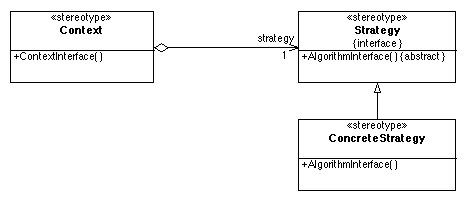
\includegraphics[width=\textwidth]{../uml/StrategyPattern.png}
	\caption{Strategie UML}
	\floatfoot{Source: (Perseo~commonswiki, Commons-Wiki, 11 Jul 2017)}
\end{figure}

\newpage
\subsection{Dekorierer}

\textit{engl. Decorator pattern}

\begin{defi}
	Der Dekorierer fügt Objekten dynamisch Funktionalität hinzu.
\end{defi}

\begin{ex}[Java]
	Im folgenden Beispiel werden wir Eis mit Extras "dekorieren".
	
	
	\lstinputlisting[language=Java, caption=Erstellen userer zu dekorierenden Schnittstelle Schnittstelle]{../java/examples/decorator/IceCream.java}
	\lstinputlisting[language=Java, caption=Schnittstellen Implementierung]{../java/examples/decorator/GenericIceCream.java}
	\lstinputlisting[language=Java,caption=Dekorierer]{../java/examples/decorator/IceCreamDecorator.java}
	\lstinputlisting[language=Java,caption=Konkrete Implementierung des Dekorierers]{../java/examples/decorator/WithChocolateChips.java}
	\lstinputlisting[language=Java,caption=Weitere konkrete Implementierung des Dekorierers]{../java/examples/decorator/WithCaramel.java}
	\lstinputlisting[language=Java, caption=Verwendung]{../java/examples/decorator/Main.java}
	
\end{ex}

\begin{why}
	Wenn Zusatzoperationen welche nur teilweise auftreten auf weitere Objekte delegiert werden sollen, während alte Objekte Fortbestand haben sollen.
\end{why}
\begin{figure}[H]
	\centering
	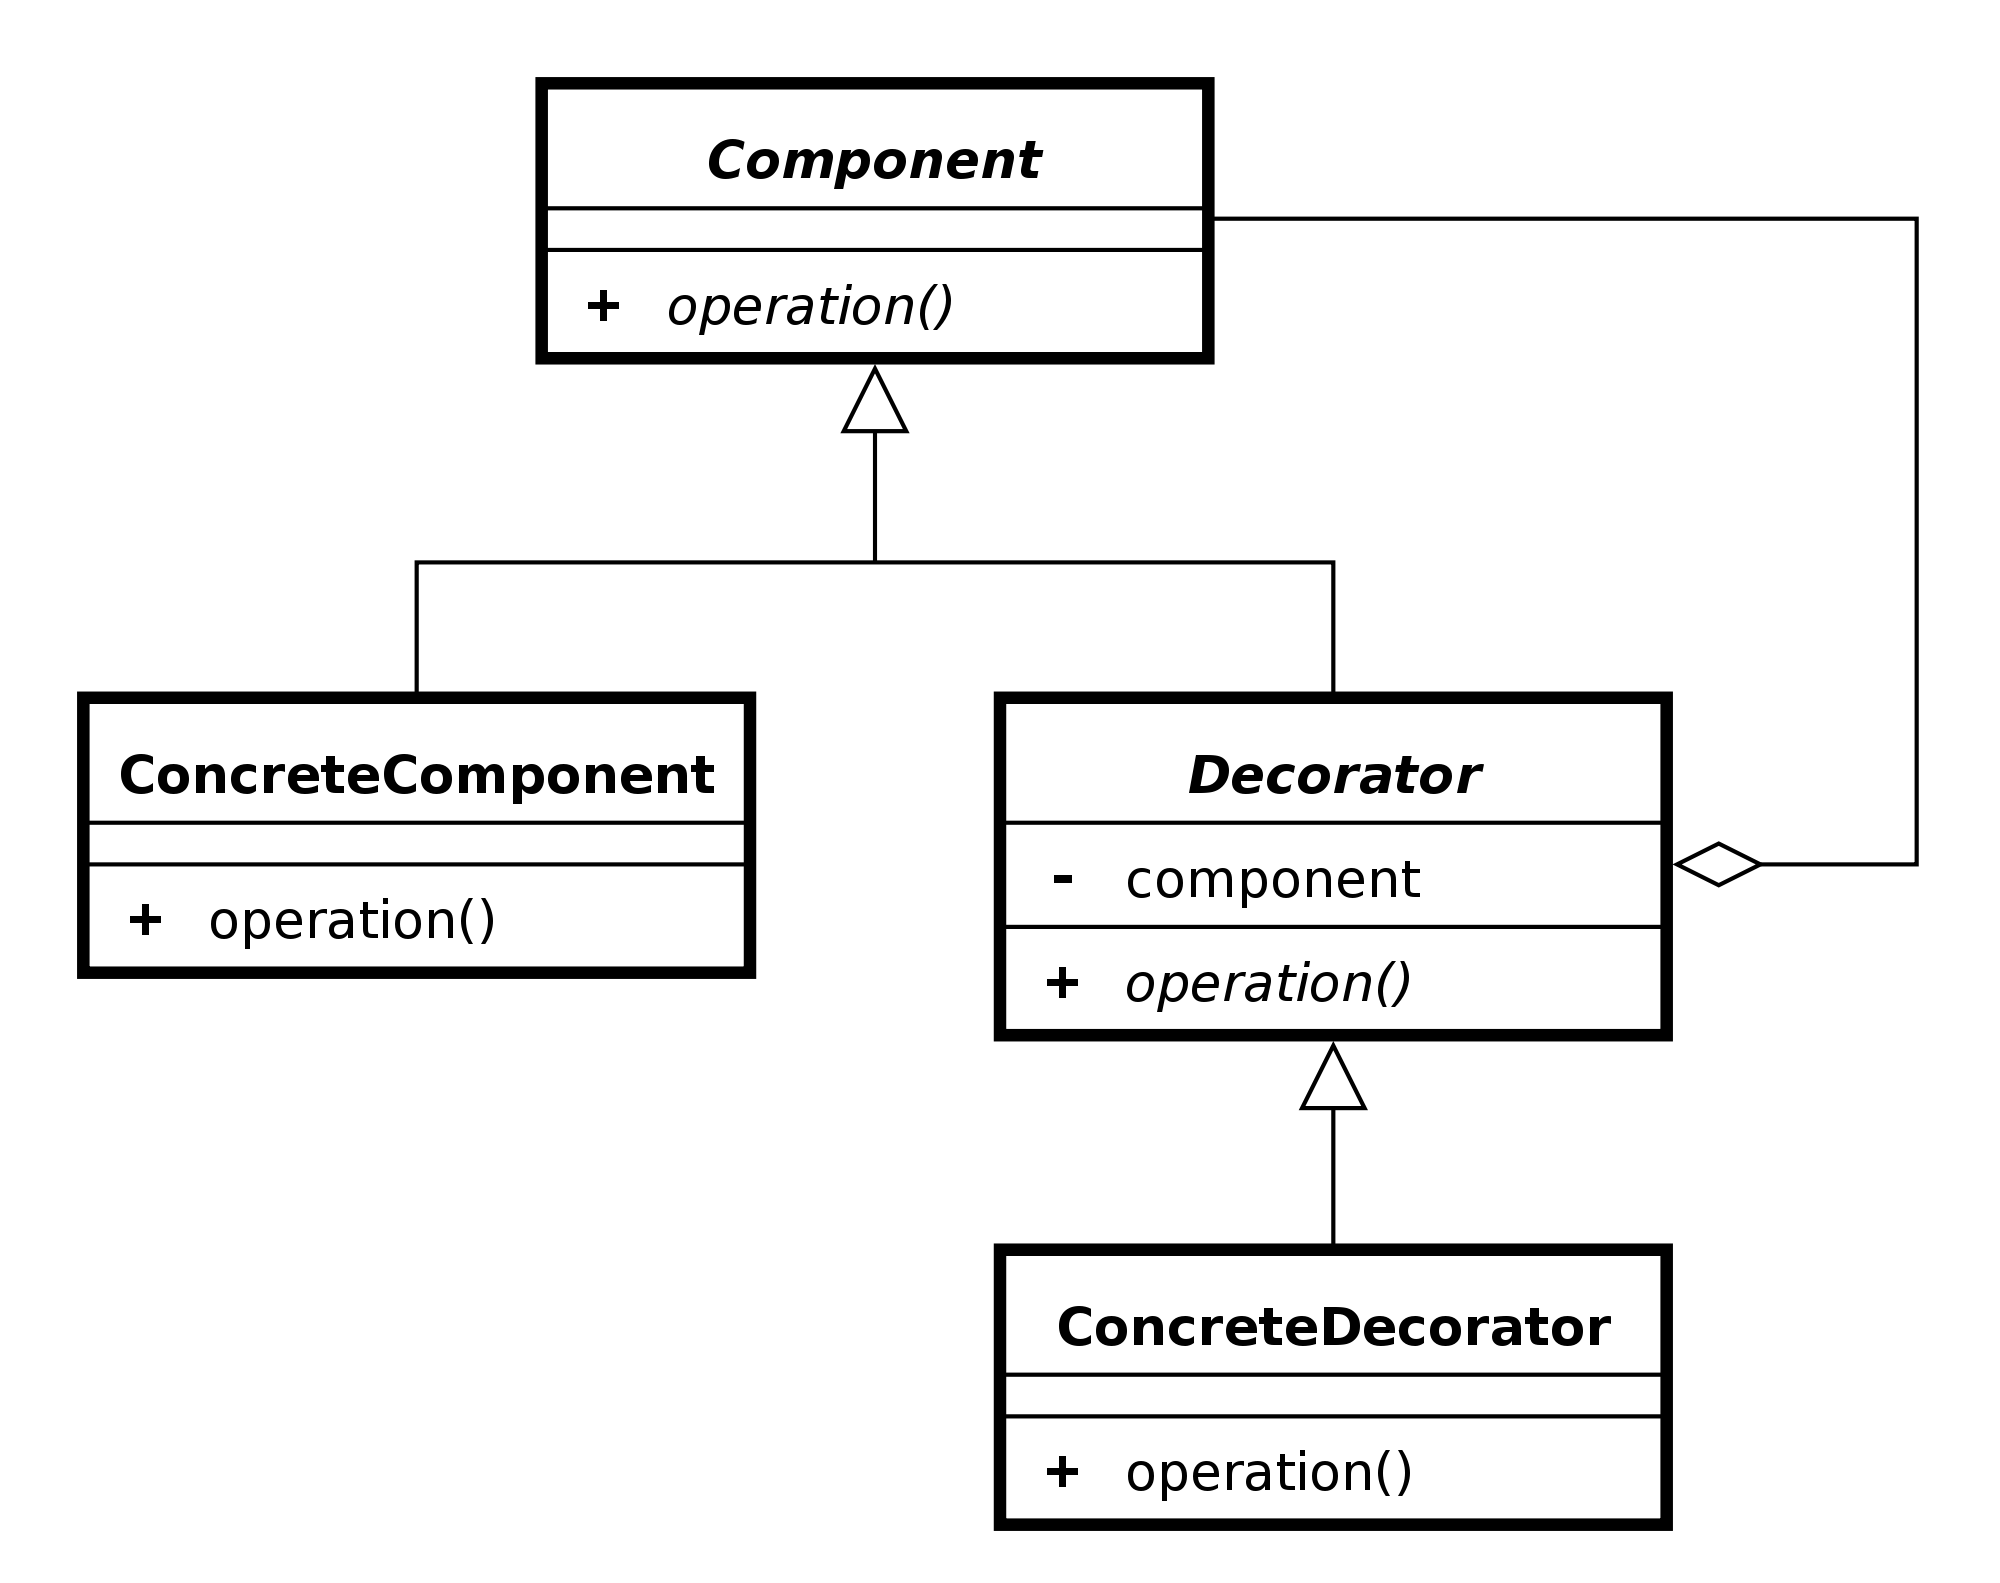
\includegraphics[width=\textwidth]{../uml/DecoratorPattern.png}
	\caption{Dekorierer UML}
\end{figure}

\newpage
\subsection{Kompositum}

\textit{engl. Composite pattern}

\begin{defi}
	Ein Kompositum ist eine Gruppe von Objekten, welche genauso behandelt wird wie eine einzelne Instanz des selben Objekttypen
\end{defi}

\begin{ex}[Java API: JComponent]
	In der Java API enthalten ist der JComponent, welcher wiederum weitere Components enthalten kann.
	Zum Beispiel kann ein JPanel ein Label und ein weiteres Panel mit einem Button und einem Bild enthalten und trotzdem wird das obere JPanel genauso als JComponent behandelt wie die einzelnen enthaltenen JComponents behandelt werden (würden).
\end{ex}

\begin{why}
	Wenn Unterscheide zwischen einer einzelnen Ausführung einer Klasse und einer Zusammensetzung dieser für die Verwendung nicht von Relevanz sind.
\end{why}
\begin{figure}[H]
	\centering
	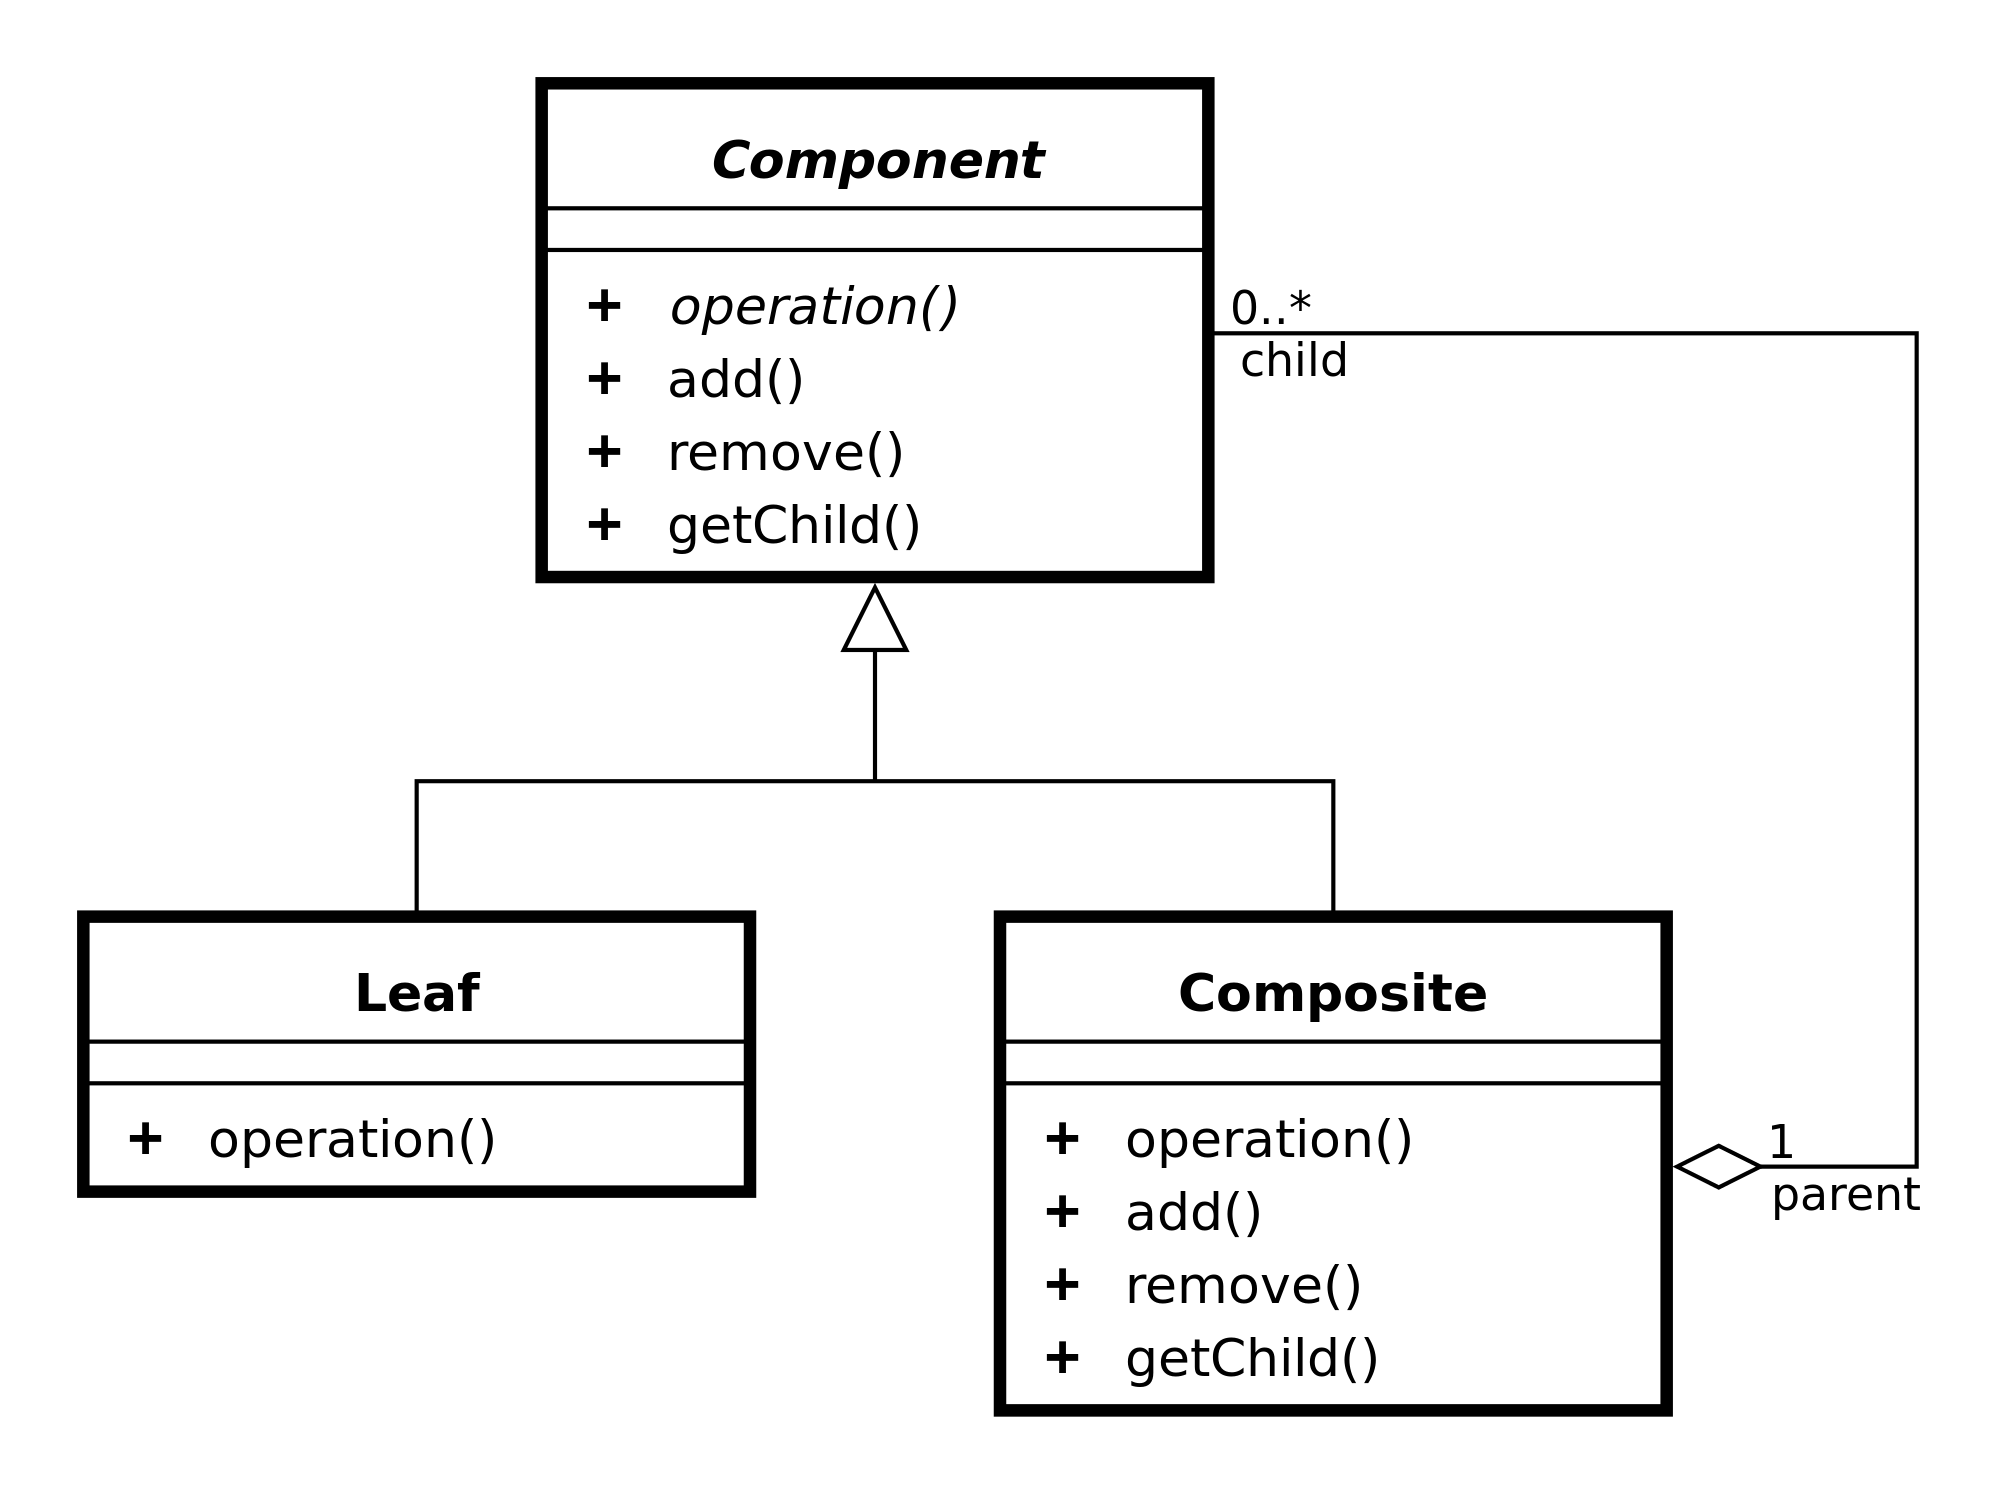
\includegraphics[width=\textwidth]{../uml/CompositePattern.png}
	\caption{Kompositum UML}
\end{figure}

\newpage
\subsection{Fabrikmethode}

\textit{engl. Factory Method}

\begin{defi}
	Eine abstrakte Klasse zur Instanziierung neuer Objekte, welche die konkrete Auswahl der konkreten zu instanziierenden Klasse seinen Unterklassen überlässt.
\end{defi}

\begin{ex}[Java]
	Im folgenden Beispiel werden wir Typen von Studenten ihre Smartphones "bauen" lassen. (Studenten bauen i.A. keine Smartphones, aber es musste ja Beispiel her)

	\lstinputlisting[language=Java, caption=Erstellen unserer Schnittestelle\, von welcher die Subklassen durch die Frabrikmethode gebaut werden sollen Schnittstelle]{../java/examples/factorymethod/Smartphone.java}
	\lstinputlisting[language=Java, caption=1. Schnittstellen Implementierung]{../java/examples/factorymethod/GenericSmartphone.java}
	\lstinputlisting[language=Java, caption=2. Schnittstellen Implementierung]{../java/examples/factorymethod/uPhone.java}
	\lstinputlisting[language=Java,caption=Abstrakte Klasse\, welche durch Fabrikmethode Objekte bauen soll]{../java/examples/factorymethod/Student.java}
	\lstinputlisting[language=Java,caption=Konkrete Implementierung der Klasse mit Fabrikmethode]{../java/examples/factorymethod/NormalStudent.java}
	\lstinputlisting[language=Java,caption=Weitere Implementierung der Klasse mit Fabrikmethode]{../java/examples/factorymethod/BusinessStudent.java}
	\lstinputlisting[language=Java, caption=Verwendung]{../java/examples/factorymethod/Main.java}
\end{ex}

\begin{why}
	\begin{enumerate}
		\item 	Wenn eine Klasse die ihre benötigten zu instanziierenden Objekte nicht kennen kann.
		\item Wenn eine Klasse benötigt, dass ihre Unterklassen Kontrolle über die konkrete Auswahl eines Objekttyps haben müssen.
		\item Zur Insanziierung eines konkreten Objektes welche das Schablonenmethoden Muster verwendet
	\end{enumerate}
\end{why}
\begin{figure}[H]
	\centering
	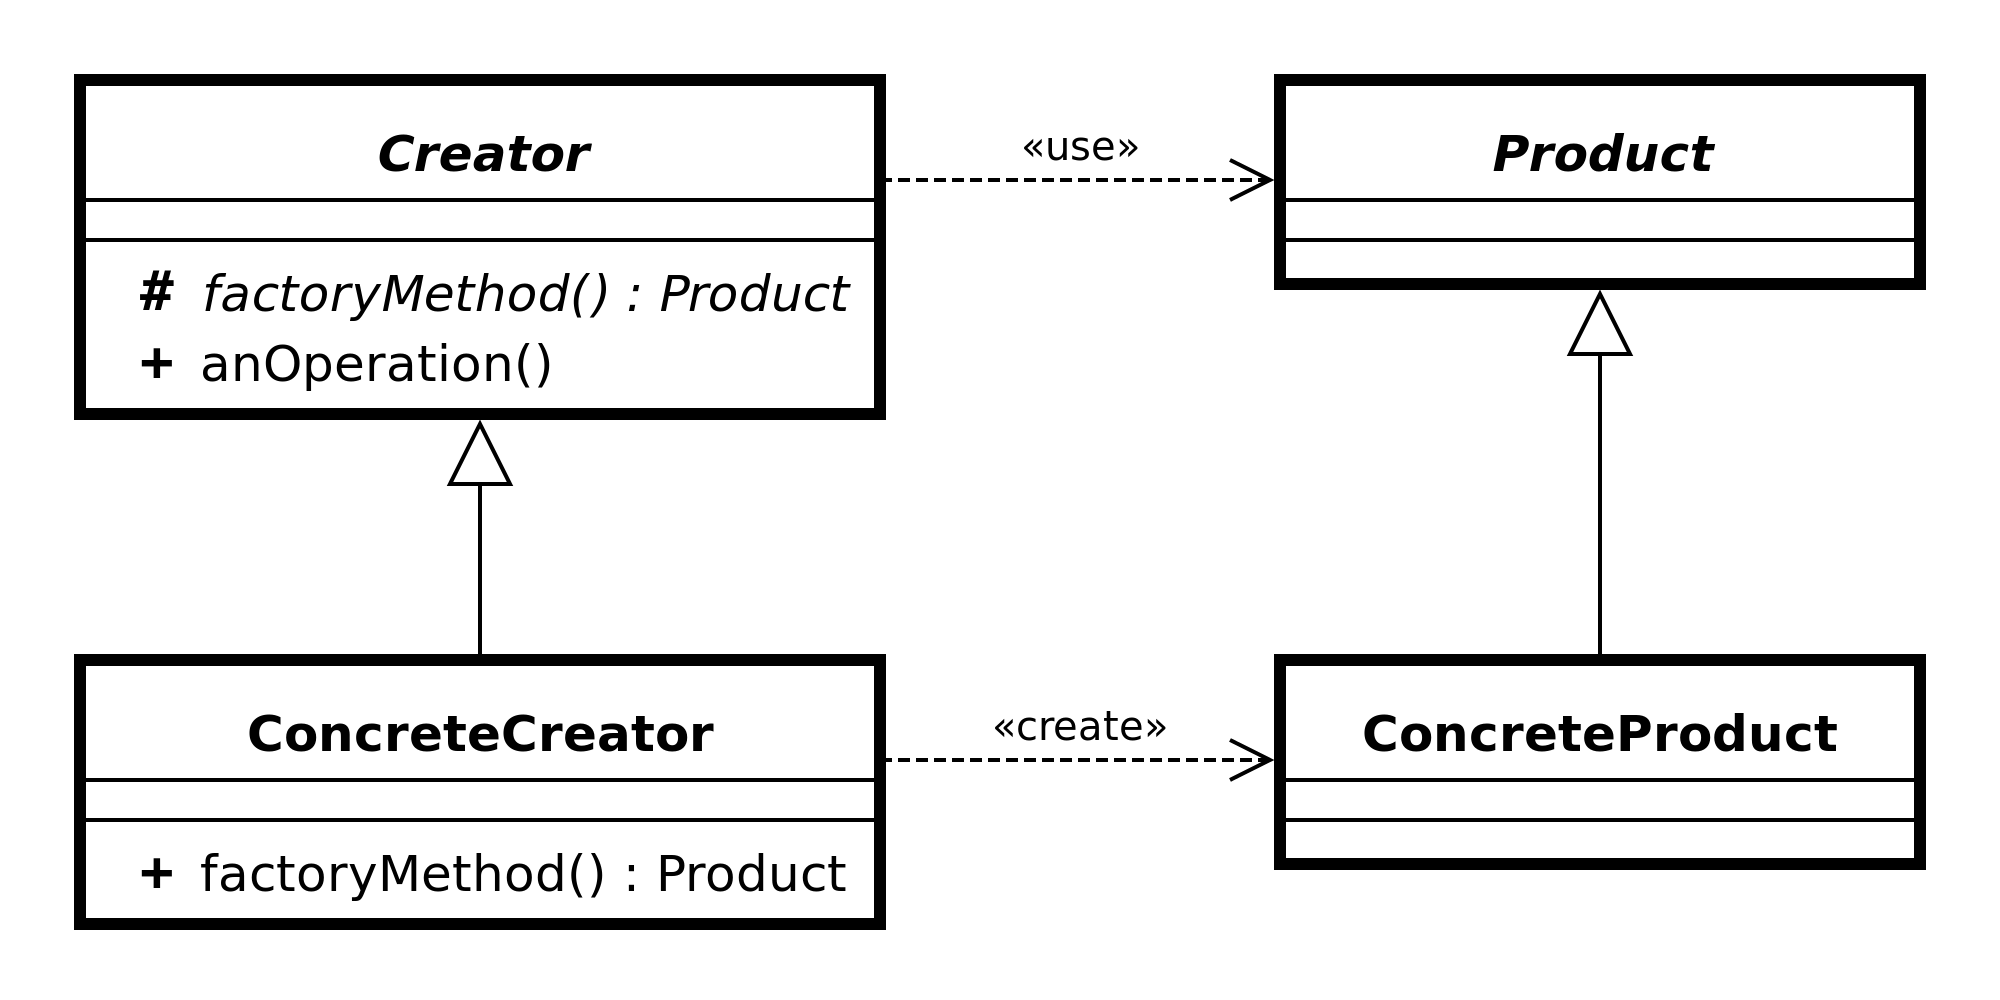
\includegraphics[width=\textwidth]{../uml/FactoryMethodPattern.png}
	\caption{Fabrikmethode UML}
\end{figure}


\newpage
\subsection{Schablonen Methode}

\textit{engl. Template Method}

\begin{defi}
	Eine Algorithmen Skelett in einer Operation, welches manche Schritte seien Unterklassen überlässt. (Zu deutsch: Eine Schablonenmethode definiert die Schritte eines Algorithmus, aber überlässt (Teil-)Implementierungen den Unterklassen)
\end{defi}

\begin{ex}[Java]
	Im folgenden Beispiel wollen wir Mate Tee und Kaffee kochen. Folgendes Beispiel wurde adaptiert von E. Freeman, et. al; Head First Design Patterns.
	
	\lstinputlisting[language=Java, caption=Abstrakte Klasse mit Algorithmus\, welcher nicht alle Schritte implementiert]{../java/examples/templatemethod/CaffeineBeverage.java}
	\lstinputlisting[language=Java, caption=1. Konkrete Umsetzung der Klasse mit Schablonenmethode]{../java/examples/templatemethod/MateTea.java}
	\lstinputlisting[language=Java, caption=2. Konkrete Umsetzung der Klasse mit Schablonenmethode]{../java/examples/templatemethod/Coffee.java}
	\lstinputlisting[language=Java, caption=Verwendung]{../java/examples/templatemethod/Main.java}
	
\end{ex}

\begin{why}
		Um einen Algorithmus zu kapseln, für welchen manche Schritte allerdings nicht allgemein implementiert werden sollen/können.	
\end{why}
\begin{figure}[H]
	\centering
	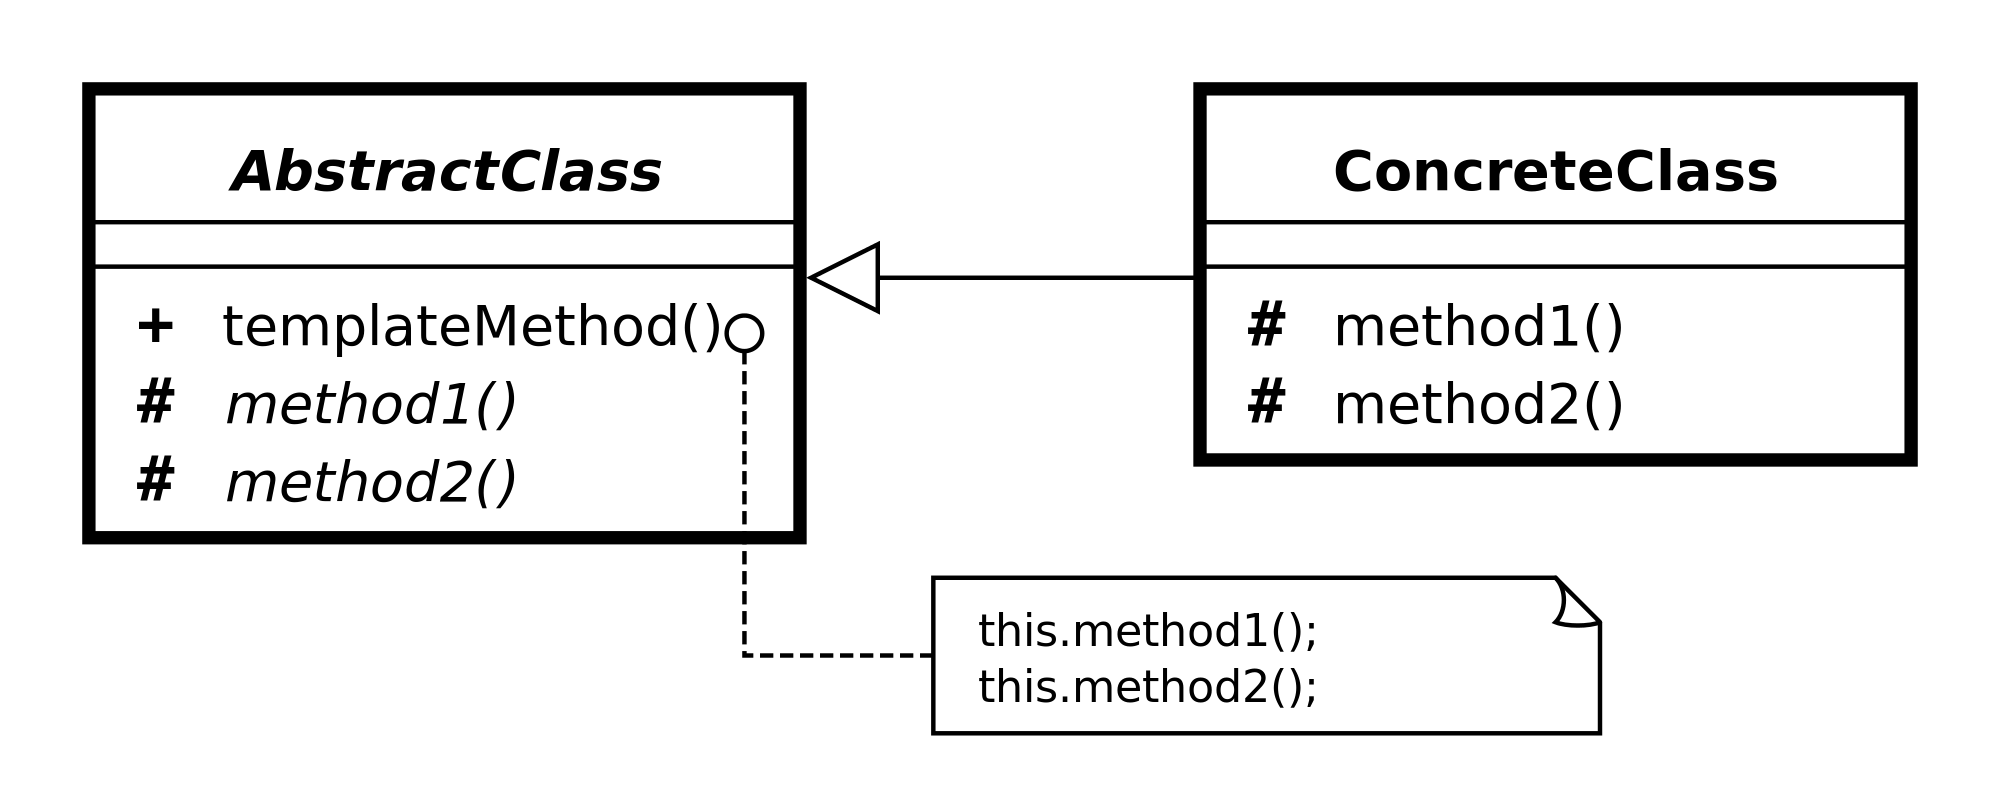
\includegraphics[width=\textwidth]{../uml/TemplateMethodPattern.png}
	\caption{Schablonenmethode UML}
\end{figure}


\newpage
\subsection{Besucher}

\textit{engl. Visitor}

\begin{defi}
	Die Kapselung eines auf einer Objektstruktur ausführenden Algorithmus von dieser.
\end{defi}

\begin{ex}[Java]
	Im folgenden Beispiel besuchen wir einen Computer auf verschiedene Arten
	
	\lstinputlisting[language=Java, caption=Zu besuchendes Interface]{../java/examples/visitor/ComputerComponent.java}
	\lstinputlisting[language=Java, caption=Konkrete Umsetzung der zu besuchenden Schnittstelle]{../java/examples/visitor/Computer.java}
	\lstinputlisting[language=Java, caption=Konkrete Umsetzung der zu besuchenden Schnittstelle]{../java/examples/visitor/CPU.java}
	\lstinputlisting[language=Java, caption=Konkrete Umsetzung der zu besuchenden Schnittstelle]{../java/examples/visitor/RAM.java}
	\lstinputlisting[language=Java, caption=Konkrete Umsetzung der zu besuchenden Schnittstelle]{../java/examples/visitor/GraphicsCard.java}
	
	\lstinputlisting[language=Java, caption=Visitorinterface]{../java/examples/visitor/ComputerComponentVisitor.java}
	\lstinputlisting[language=Java, caption=Konkrete Umsetzung der besuchenden Schnittstelle]{../java/examples/visitor/FixVisitor.java}
	\lstinputlisting[language=Java, caption=Konkrete Umsetzung der besuchenden Schnittstelle]{../java/examples/visitor/SpillVisitor.java}
	
	\lstinputlisting[language=Java, caption=Verwendung]{../java/examples/visitor/Main.java}
	
\end{ex}

\begin{why}
	Um das Open-Closed Principle einzuhalten.
\end{why}
\begin{figure}[H]
	\centering
	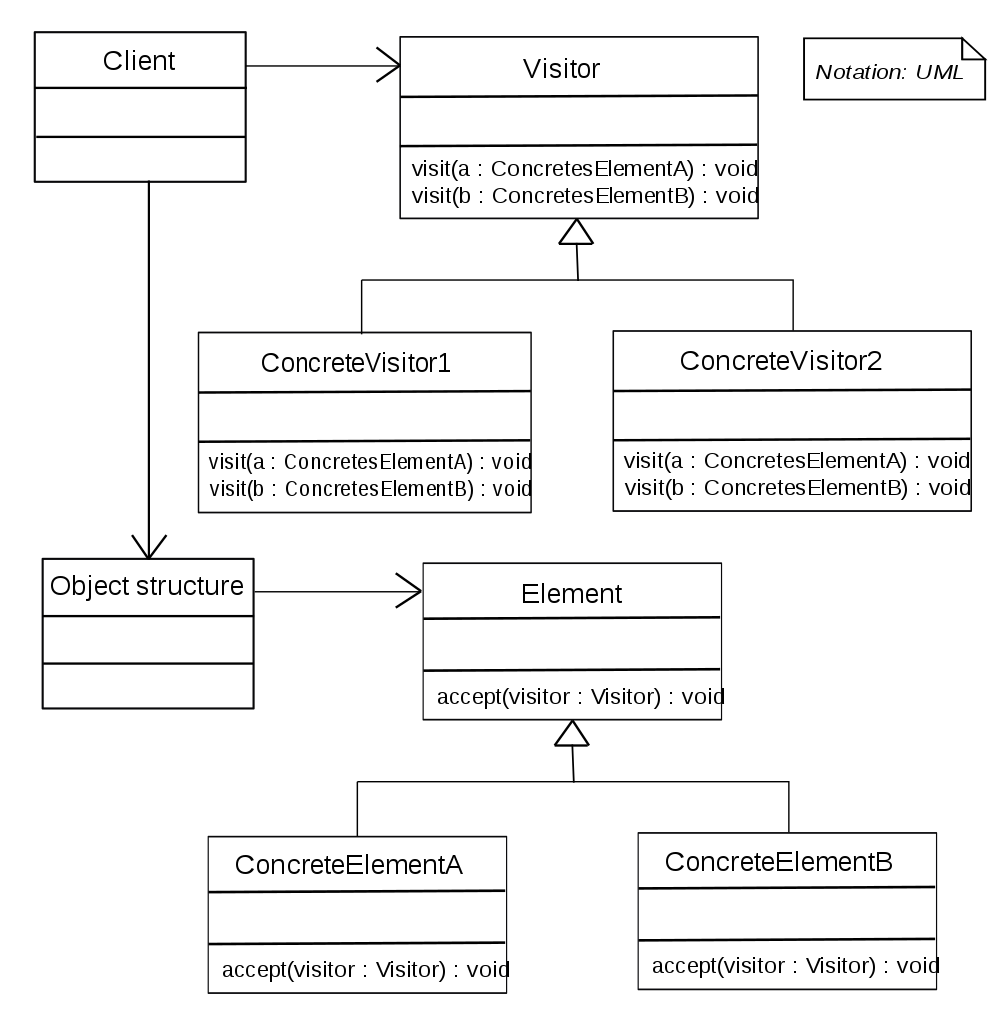
\includegraphics[width=\textwidth]{../uml/VisitorPattern.png}
	\caption{Besucher UML}
	\floatfoot{Source: (Sae1962, Commons-Wiki, 11 Jul 2017)}
\end{figure}




\newpage
\subsection{Abstrakte Fabrik}

\textit{engl. Abstract Factory}

\begin{defi}
	Eine Abstrakte Fabrik bietet eine Schnittstelle zur Instanziierung von Familien bestehend aus voneinander abhängigen Objekten
\end{defi}

\begin{ex}[Java]
	Im folgenden Beispiel besuchen wir einen Computer auf verschiedene Arten
	
	\lstinputlisting[language=Java, caption=Die abstrakte Fabirk]{../java/examples/abstractfactory/GUIFactory.java}
	\lstinputlisting[language=Java, caption=Konkrete Umsetzung der Fabrik]{../java/examples/abstractfactory/OSXGUIFactory.java}
	\lstinputlisting[language=Java, caption=Konkrete Umsetzung der Fabrik]{../java/examples/abstractfactory/LinuxGUIFactory.java}
	\lstinputlisting[language=Java, caption=Konkrete Umsetzung der Fabrik]{../java/examples/abstractfactory/WindowsGUIFactory.java}
	
	
	\lstinputlisting[language=Java, caption=Das zu erstellende Interface]{../java/examples/abstractfactory/NavBar.java}
	
	
	\lstinputlisting[language=Java, caption=Verwendung]{../java/examples/abstractfactory/Main.java}
	
\end{ex}

\begin{why}
	\begin{enumerate}
		\item Um eine System unabhängig von seiner Produkterzeugung sein soll
		\item Wenn eine Familie von aufeinander abgestimmten Produkten benötigt wird
		\item Bei einer Bibliothek welche keine Implementierungen, sondern nur Schnittstellen offen legen soll
	\end{enumerate}
	
	
\end{why}
\begin{figure}[H]
	\centering
	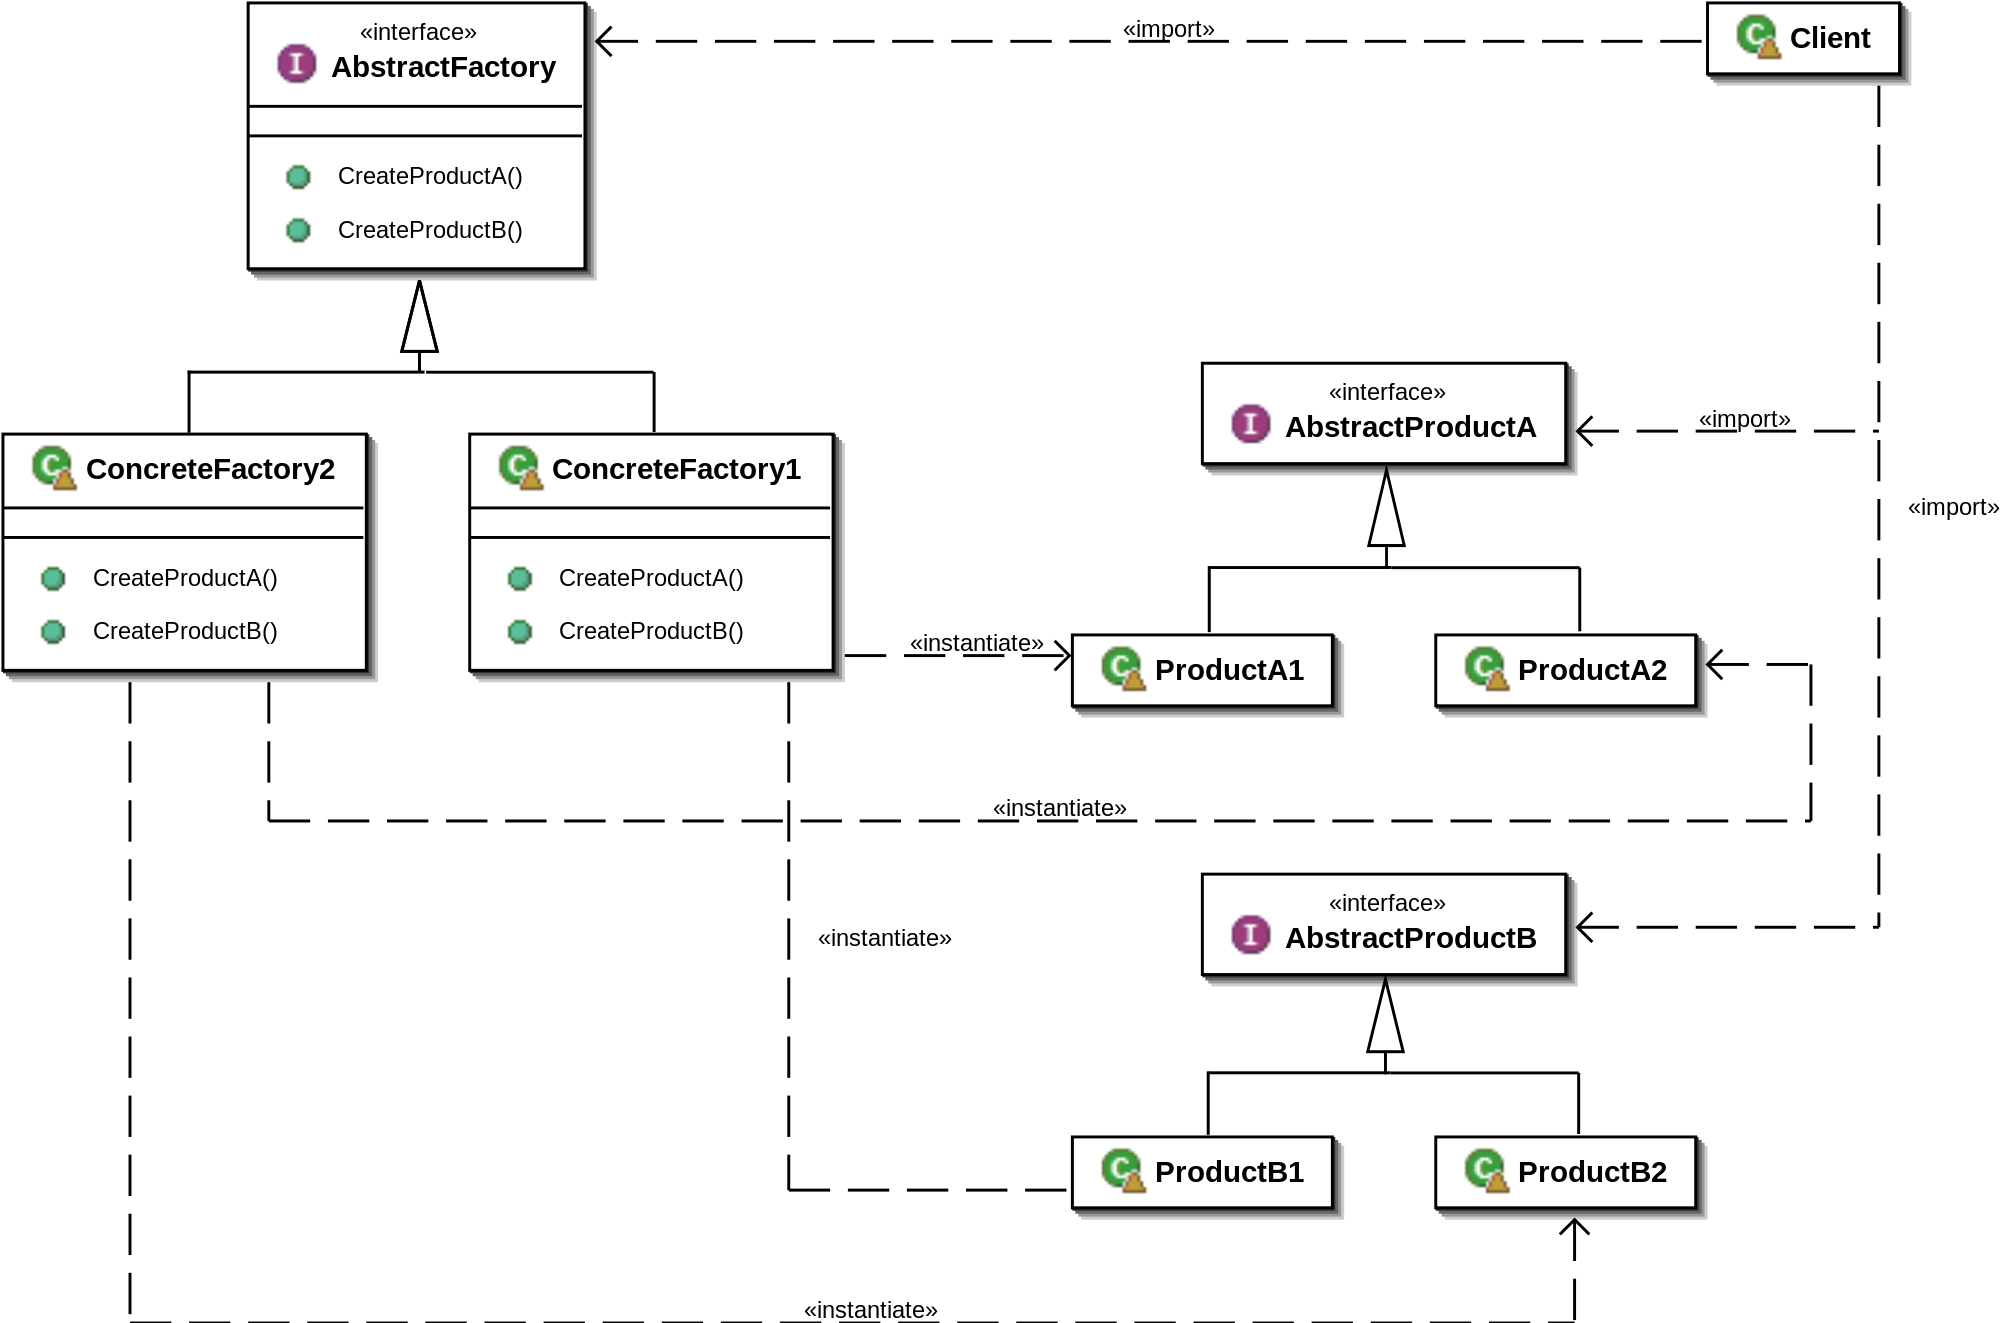
\includegraphics[width=\textwidth]{../uml/AbstractFactoryPattern.png}
	\caption{Abstrakte Fabrik UML}
	\floatfoot{Source: (Giacomo Ritucci, Commons-Wiki, 11 Jul 2017)}
\end{figure}

\newpage
\appendix
\section{Abbilungsübersicht}
\listoffigures


	
\end{document}